\documentclass[../../main.tex]{subfiles}
\begin{document}
\section{Experiments}

To access efficiency of both algorithms, and their MapReduce frameworks set of experiements was performed on the data just described. Two different forms of tests were performed; some for measuring the precision of the algorithms, and some for measuring the speed of the algorithms.\\

For all experiments, $\epsilon=0.95$. The {\bf MM} clustering algorithm will be refered to as {\bf MM}, likewise will the {\bf MM½} clustering algorithm be referred to as {\bf MM½}. 
\subsection{Precision tests}

In Eq. \ref{minmaxerror}, a metric of the error was set up for the number of hash functions $H$. This error did not provide an answer to relation between $H$ and the size of $k$-mers $k$ and its error. Therefore, a practical testing of this relation was performed, to investigae the precision of {\bf MM} and {\bf MM½}.\\

A gold standard was instrumental to determine the precision of our algorithms. For this purpose, the Levenshtein similarity was used, as defined in the Tools section. If two strings had a Levenshtein similarity above $\epsilon$ they were placed in the same cluster. The gold standard, \textbf{GS}, were then set to be the number of clusters found by the Levenshtein similarity clustering algorithm. Once the \textbf{GS} were retrieved, the error of an algorithms' found number of clusters, $C$, could be defined as the difference between $C$ and the gold standard \textbf{GS}
$$
E = | C - \mathbf{GS}|
$$

similarly, the percentage of error $E_p$ was 
$$
E_p = \frac{|C - \mathbf{GS}|}{\mathbf{GS}}
$$

The lower $E$ was, the more precise the algorithm. As both {\bf MM} and {\bf MM½} results depend on $k$ and $H$, a large set of tests were performed to determine the precision of each algorithm at many $k$ and $H$. When the optimal settings were found, the results could then be compared to \texttt{uClust} algorithm's precision. 
\subsubsection{MM precision tests}
First, the {\bf MM} algorithm's precision tests were made. In order to narrow down the number of $k$ and $H$ to test, a heat plot of a wide set of $k$ and $H$ for seeing the big scope was made, as seen in Fig. \ref{fig:wideC}. From this wide study, ostensibly the error increased rapidly at $k>13$, and $k<5$ were less precise than $k=5$. Also, at $H>80$ the error seemed to stop changing significantly.

\begin{figure}[H]
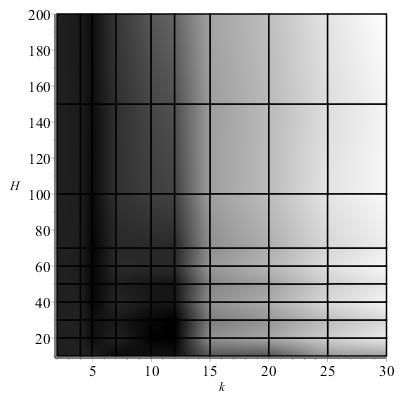
\includegraphics[scale=0.5]{precision/minmax/cecum1wide.jpg}
\caption{Heat map of the error of {\bf MM} at a widely dispersed array of $k$ and $H$, run on \texttt{Cecum1}. Darkness increases as the error decreases.}\label{fig:wideCminmax}
\end{figure}

The results of this test showed that the more rigourous tests could be performed at a more narrow set of $k$ and $H$, as seen in Fig. \ref{fig:Cpreciseminmax}. All heat maps showed very similar results for all samples. There were specific areas that seemed to have repeatedly have a very low error, specifically at
\begin{itemize}
\item $k$=5, a black line from $H=50$ to $H=80$.
\item $k=6$, two black spots at around $H=10$ and $H=22$.
\item $k=10,11,12$, two big black spots at around $H=16$ and $H=30$. 
\end{itemize}
These areas of interest were deemed to be most precise. Therefore, each was tested alongside \texttt{uClust}, to be able to compare them to each other. Fig. \ref{fig:allKminmax} shows the results of these tests.\\

Fig. \ref{fig:allKminmax}(a) shows that at $k=5$, the overall performace of the algorithm appeared near comparable to \texttt{uClust}, with a maximum error of approx. 33\%. At the spikes, the precision is even higher than \texttt{uClust}, most notably at $H=54$, $H=65$ and $H=66$, where the average error over all samples was around 4\%. 

Fig. \ref{fig:allKminmax}(b) shows that at $k=6$, the maximal error is around 70\%, much worse than that of \texttt{uClust}. However, two spikes also appeared here at $H=13$ and $H=22$, both with an average error of around 7\%, slightly better than \texttt{uClust}.\\

Fig. \ref{fig:allKminmax}(c-e) show that in spite of generally portraying a high error overall at $k=10,11,12$, reaching maximum errors of over 80\%, they still had potentially low errors; Most notably at $k=10,H=20$, $k=11,H=30$, and $k=12,H=30$, with spikes with an average error about 10\%, about the same as \texttt{uClust}.\\

\begin{figure}[H]
\begin{subfigure}[b]{.5\textwidth}
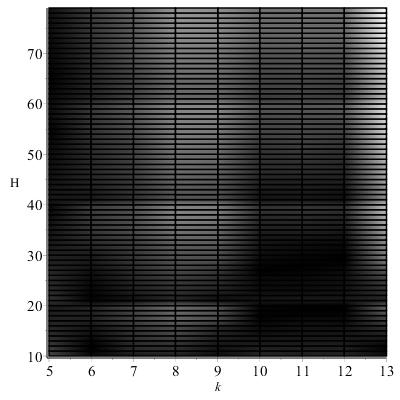
\includegraphics[width=\textwidth]{precision/minmax/cecum1precise}
\caption{\texttt{Cecum1}}
\end{subfigure}
\begin{subfigure}[b]{.5\textwidth}
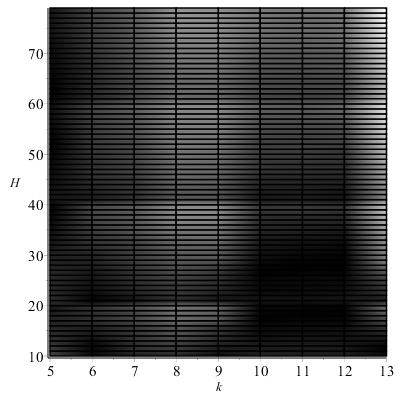
\includegraphics[width=\textwidth]{precision/minmax/cecum2precise}
\caption{\texttt{Cecum2}}
\end{subfigure}
\begin{subfigure}[b]{.5\textwidth}
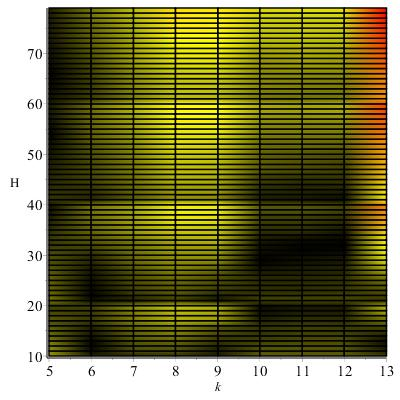
\includegraphics[width=\textwidth]{precision/minmax/cecum3precise}
\caption{\texttt{Cecum3}}
\end{subfigure}
\begin{subfigure}[b]{.5\textwidth}
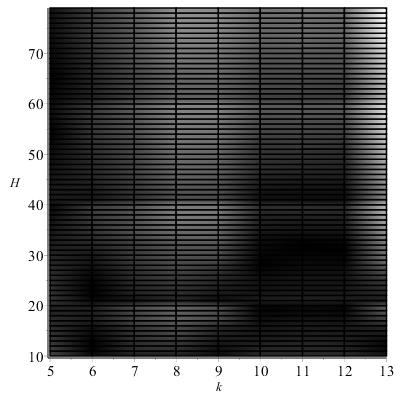
\includegraphics[width=\textwidth]{precision/minmax/cecum4precise}
\caption{\texttt{Cecum4}}
\end{subfigure}
\begin{subfigure}[b]{.5\textwidth}
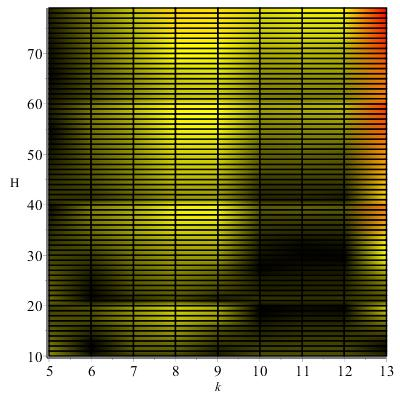
\includegraphics[width=\textwidth]{precision/minmax/cecum5precise}
\caption{\texttt{Cecum5}}
\end{subfigure}
\caption{Heat maps of the error of {\bf MM} at a narrow array of $k$ and $H$ at all 5 samples of \texttt{Cecum} DNA. Darkness increases as the error decreases.}\label{fig:Cpreciseminmax}
\end{figure}

\begin{figure}[H]
\begin{subfigure}[b]{.5\textwidth}
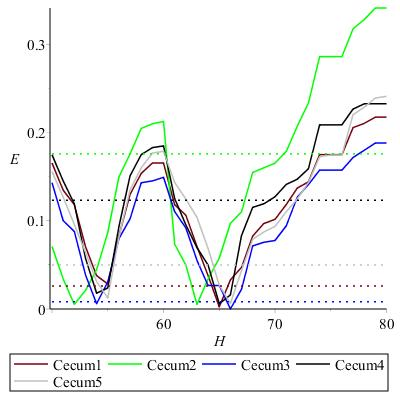
\includegraphics[width=\textwidth]{precision/minmax/k5cecum}
\caption{\texttt{k=5}}
\end{subfigure}
\begin{subfigure}[b]{.5\textwidth}
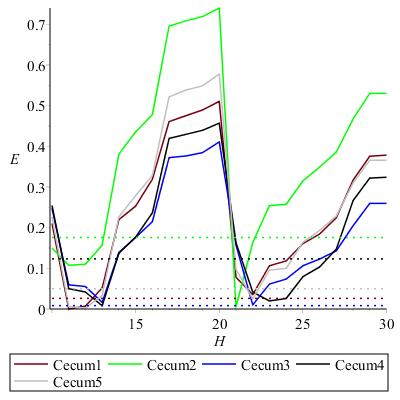
\includegraphics[width=\textwidth]{precision/minmax/k6cecum}
\caption{\texttt{k=6}}
\end{subfigure}
\begin{subfigure}[b]{.5\textwidth}
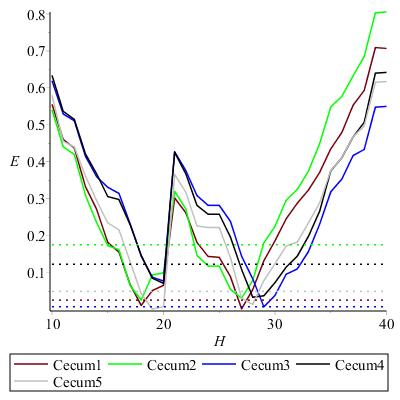
\includegraphics[width=\textwidth]{precision/minmax/k10cecum}
\caption{\texttt{k=10}}
\end{subfigure}
\begin{subfigure}[b]{.5\textwidth}
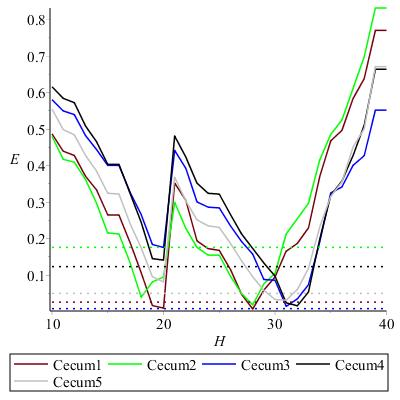
\includegraphics[width=\textwidth]{precision/minmax/k11cecum}
\caption{\texttt{k=11}}
\end{subfigure}
\begin{subfigure}[b]{.5\textwidth}
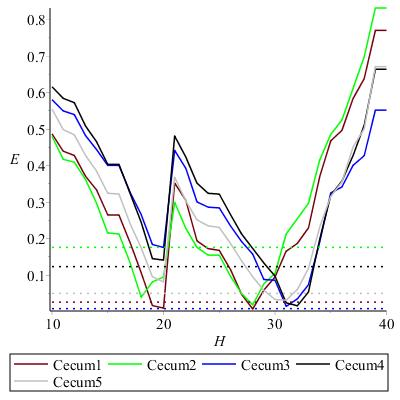
\includegraphics[width=\textwidth]{precision/minmax/k11cecum}
\caption{\texttt{k=10}}
\end{subfigure}
\caption{Plots with $H$ on the $x$-axis and error $E_p$ in percent $(0.5 = 50\%)$ the $y$-axis, each plot at different $k$. The lines in the plots signify the error at the given $k$ and $H$ of {\bf MM}, while the dotted lines signify the error of \texttt{uClust} at each file. The colours define the sample file.}
\label{fig:allKminmax}
\end{figure}

\subsubsection{MM½ precision tests}

The tests of {\bf MM½} were performed completely parallel to those of {\bf MM}, but with lower $H$ as reputedly {\bf MM½} only needs half as many hash functions as the minwise sketch\footnote{see Minwise and Maxwise Hashing Section}. In Fig. \ref{fig:wiseCminmaxhalf} figures the test of a wide array of $k$ and $H$.
\begin{figure}[H]
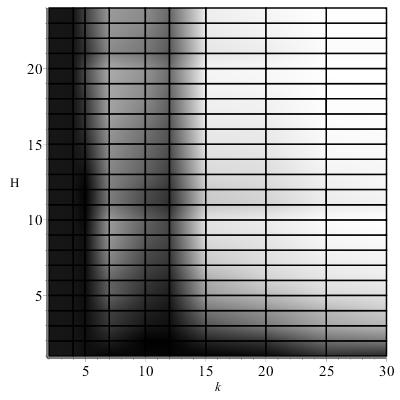
\includegraphics[scale=0.5]{precision/minmaxhalf/cecum1wide.jpg}
\caption{Heat map of the error of {\bf MM½} at a widely dispersed array of $k$ and $H$, run on \texttt{Cecum1}. Darkness increases as the error decreases.}\label{fig:wiseCminmaxhalf}
\end{figure}

The large white plateau in Fig. \ref{fig:wiseCminmaxhalf} meant that $k>15$ could be ignored, as the error at this area was very high. Similarly, $k<5$ gave more error than $k=5$ and could therefore be ignored. $H$ could be reduced to $H< 15$, as the blackest spot seems around $k=5,H=12$.\\

New tests were performed with these limitations. The results can be seen in Fig. \ref{fig:cpreciseminmaxhalf}. All five plot are almost completely identical, showing that mostly at $H=1$ and $H=2$, the precision is highest. The only exception was at $k=5$, where there seemes to be a lower error along all $H$. An additional analysis showed that the minimum error in each heat map of Fig. \ref{fig:cpreciseminmaxhalf} was always at $k=8, H=1$. This result was but a stroke of luck, since a single hash function would theoretically cause the error of the {\bf MM½} sketch to be too high to be applicable for proper comparison (see Eq. \ref{minmaxerror}).\\

For further analysis of the $k$ of interest, the errors of each file at $k=5$,$k=8$ and $k=12$ were plotted, as seen in Fig. \ref{fig:allKminmaxhalf}. Fig. \ref{fig:allKminmaxhalf}(a-c) all have maximum errors that surpass 100\%, even reaching as high as 700\% error. Only in Fig. \ref{fig:allKminmaxhalf}(a) a cuspidate spike was present at $H=12$ with an average error of 20\%, around the double of \texttt{uClust} average error.\\


\begin{figure}[H]
\begin{subfigure}[b]{.5\textwidth}
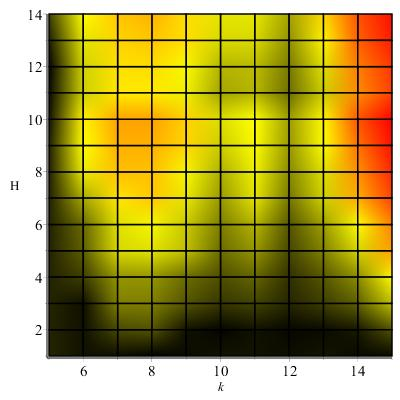
\includegraphics[width=\textwidth]{precision/minmaxhalf/cecum1precise}
\caption{\texttt{Cecum1}}
\end{subfigure}
\begin{subfigure}[b]{.5\textwidth}
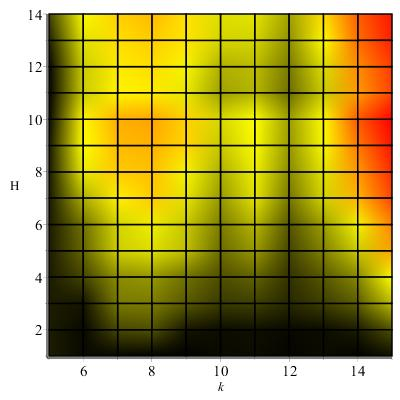
\includegraphics[width=\textwidth]{precision/minmaxhalf/cecum2precise}
\caption{\texttt{Cecum2}}
\end{subfigure}
\begin{subfigure}[b]{.5\textwidth}
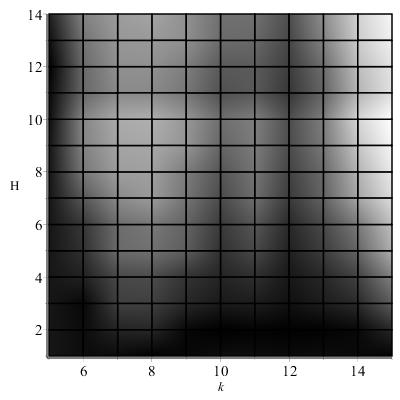
\includegraphics[width=\textwidth]{precision/minmaxhalf/cecum3precise}
\caption{\texttt{Cecum3}}
\end{subfigure}
\begin{subfigure}[b]{.5\textwidth}
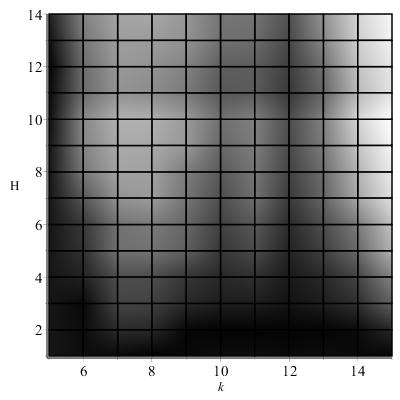
\includegraphics[width=\textwidth]{precision/minmaxhalf/cecum4precise}
\caption{\texttt{Cecum4}}
\end{subfigure}
\begin{subfigure}[b]{.5\textwidth}
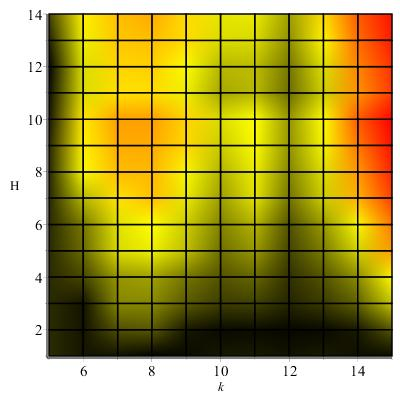
\includegraphics[width=\textwidth]{precision/minmaxhalf/cecum5precise}
\caption{\texttt{Cecum5}}
\end{subfigure}
\caption{Heat maps of the error of {\bf MM½} at a narrow array of $k$ and $H$ at all 5 samples of \texttt{Cecum} DNA. Darkness increases as the error decreases}
\label{fig:cpreciseminmaxhalf}
\end{figure}

\begin{figure}[H]
\begin{subfigure}[b]{.5\textwidth}
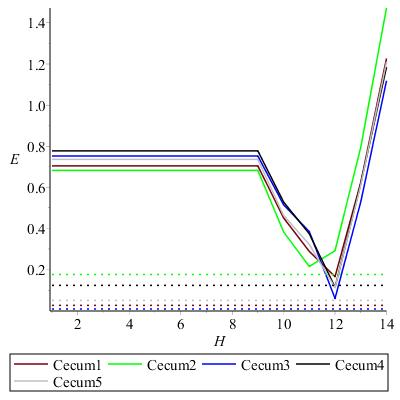
\includegraphics[width=\textwidth]{precision/minmaxhalf/k5cecum}
\caption{\texttt{k=5}}
\end{subfigure}
\begin{subfigure}[b]{.5\textwidth}
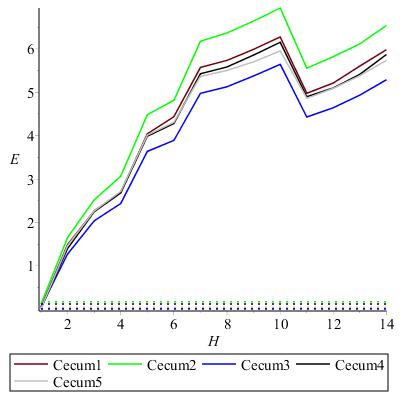
\includegraphics[width=\textwidth]{precision/minmaxhalf/k8cecum}
\caption{\texttt{k=8}}
\end{subfigure}
\begin{subfigure}[b]{.5\textwidth}
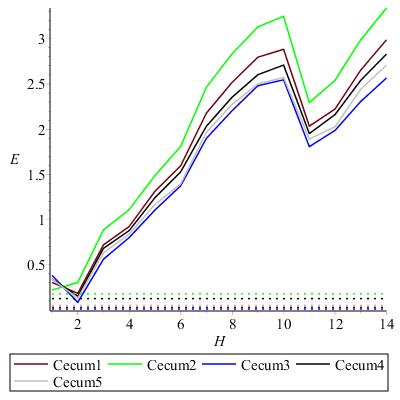
\includegraphics[width=\textwidth]{precision/minmaxhalf/k12cecum}
\caption{\texttt{k=12}}
\end{subfigure}
\caption{Plots with $H$ on the $x$-axis and error $E_p$ in percent $(0.5 = 50\%)$ on the $y$-axis, each plot at different $k$. The lines in the plots signify the error at the given $k$ and $H$ of {\bf MM½}, while the dotted lines signify the error of \texttt{uClust} at each file. The colours define the sample file.}
\label{fig:allKminmaxhalf}
\end{figure}

\subsubsection{Comparison}
To determine the precision of {\bf MM}, {\bf MM½} and \texttt{uClust}, Fig. \ref{fig:allKminmaxhalf} and Fig. \ref{fig:allKminmax} were perfect candidates. One of the most notable differences between the two graphs was the structure of the results for {\bf MM}, which took an almost "W" like form. The reason for this is from how the sketches of two sequences are compared in Eq. \ref{minmaxjaccard}. In contrast to Eq. \ref{minmaxhalfjaccard}, {\bf MM} takes advantage of the strong points of both the max- and minwise hashing by finding the intersection of jaccards. This means that if the maxwise hashing is most precise at $H=12$, and minwise is most precise at $H=23$, the spikes will appear at these two spots.\\

Comparing the two, {\bf MM} was quite simply much more precise than {\bf MM½}, by very large margin. In fact, at the most precise, {\bf MM½} at $k=5$ was still not as good as the worst {\bf MM} was at $k=5$ in our tests. In fact, {\bf MM} turned out to be even more precise than \texttt{uClust} at some very specific parameter settings of $k$ and $H$.\\

The extreme imprecision of {\bf MM½} was in fact so high, that it proved almost nonfunctional for practical purposes, if precision in any way was considered of any importance. {\bf MM} however proved that it could compete with \texttt{uClust} in terms of precision. Therefore, {\bf MM} was considered a good candidate for an alternative to \texttt{uClust}. What remained was to determine whether it could compare speed-wise.

\subsection{Speed tests}

For testing the speed, the MapReduce Framework using Pig Scripts were taken in use for {\bf MM} and {\bf MM½}. \texttt{uClust} was run with the setting: \texttt{cluster\_fast input -id 0.95 -uc output} as storing is also included in the Pig Scripts. As only the 32 bit version of \texttt{uClust} was available, there was a memory limit to the size of the operation. For this reason, some of the sample files could not be finished by \texttt{uClust}; this occurence will be noted as Mem. Exed.\\

To achieve the highest speed without loss of too much precision, the precision tests were used to determine the optimal parameters. {\bf MM} was run at $k=6$ and $H=13$, which as seen in Fig. \ref{fig:allKminmax}(b) is comparable to \texttt{uClust} in terms of precision. {\bf MM½} was run with $k=5$ and $H=12$.\\

The results of the test can be seen in Table \ref{tab:speedtest}. As expected, {\bf MM½} was consequently faster than {\bf MM}. Theoretically, {\bf MM½} should be twice as fast as {\bf MM}. This turned out true in all cases except for the runtime of \texttt{Actino1mio} and \texttt{Actino500K}. Here {\bf MM½} was 10 times faster than {\bf MM}, caused by the fact that fewer clusters were produced by {\bf MM½}. Therefore the outer loop of the {\bf MM½} greedy algorithm iterated less times than the outer loop of {\bf MM}. Such a difference in speed was not predicted, but says more about the imprecision of {\bf MM½} than the algorithms' relative speed.\\

The reason why {\tt uClust} was faster in both {\tt Silva50K} and {\tt Actino50K} laid in that the MapReduce Framework had a long startup time\footnote{see section about MapReduce}. If we had used a single node version of {\bf MM} and {\bf MM½}, we could probably have achieved much higher speeds at samples sizes of 50000 and less, since it would have no startup time. The MapReduce Framework would therefore first be advantageous to a single node solution using input files with 100.000 sequences or more.\\

Overall, there was a duality of speed between the two sample sets. In the \texttt{Actino} sample set, \texttt{uClust} consistently ran faster than both {\bf MM} and {\bf MM½}, with an increasing difference in speed over sample size. In the \texttt{Silva} samples, both {\bf MM} and {\bf MM½} ran faster than \texttt{uClust} at sample size higher than {\tt Silva50K}. In fact, {\bf MM} was almost twice as fast as \texttt{uClust} on the run of \texttt{Silva500K}, and the difference in speed increased with sample size.\\

While the frequency of cases where {\bf MM} and {\bf MM½} are faster than {\tt uClust} remains unknown, occasionally {\bf MM} and {\bf MM½} trumps \texttt{uClust}. In choosing between {\bf MM½} and {\bf MM}, a strong case could be made for {\bf MM}. {\bf MM½} may have been double as quick as {\bf MM}, but this at the cost of precision. So much precision, that one goes from statistically useless using {\bf MM½} to competing with \texttt{uClust} using {\bf MM}. And since {\bf MM} was also quicker than {\tt uClust} in some cases, the results suggest that it could serve as a good alternative to \texttt{uClust}.\\


\begin{table}[H]
\centering
\begin{tabular}{l l l l}
\hline
 & \multicolumn{3}{c}{runtime of sample in $s$}\\
\textbf{Sample} & \textbf{uClust} & \textbf{MM} & \textbf{MM½} \\
\hline \\
\texttt{Actino50K} & 2.0 & 18.3 & 13.6 \\
\texttt{Actino100K} & 5.0 & 23.2 & 18.7 \\
\texttt{Actino200K} & 9.0 & 53.4 & 28.8 \\
\texttt{Actino500K} & 14.0 & 208.4 & 58.3 \\
\texttt{Actino1mio} & Mem. Excd. & 1033.8 & 103.3 \\
\texttt{Silva50K} & 16.0 & 18.3 & 13.6\\
\texttt{Silva100K} & 33.0 & 28.3 & 18.3\\
\texttt{Silva200K} & 70.0 & 48.6 & 33.5\\
\texttt{Silva500K} & 208.0 & 133.5 & 68.3\\
\texttt{Silva1mio} & Mem. Excd. & 273.9 & 128.5\\
\hline
\end{tabular}
\caption{Comparison of clustering speed of three algorithms on 10 samples. \texttt{uClust} is run with \texttt{cluster\_fast} option, {\bf MM} with $k=6$ and $H=13$, {\bf MM½} has $k=5$ and $H=12$. The runtime the clustering speed is given in seconds.}\label{tab:speedtest}
\end{table}


\end{document}

